\section{Results}
\label{sec:c3_results}

% One orbit is 49.5 s

\begin{figure}
\centering
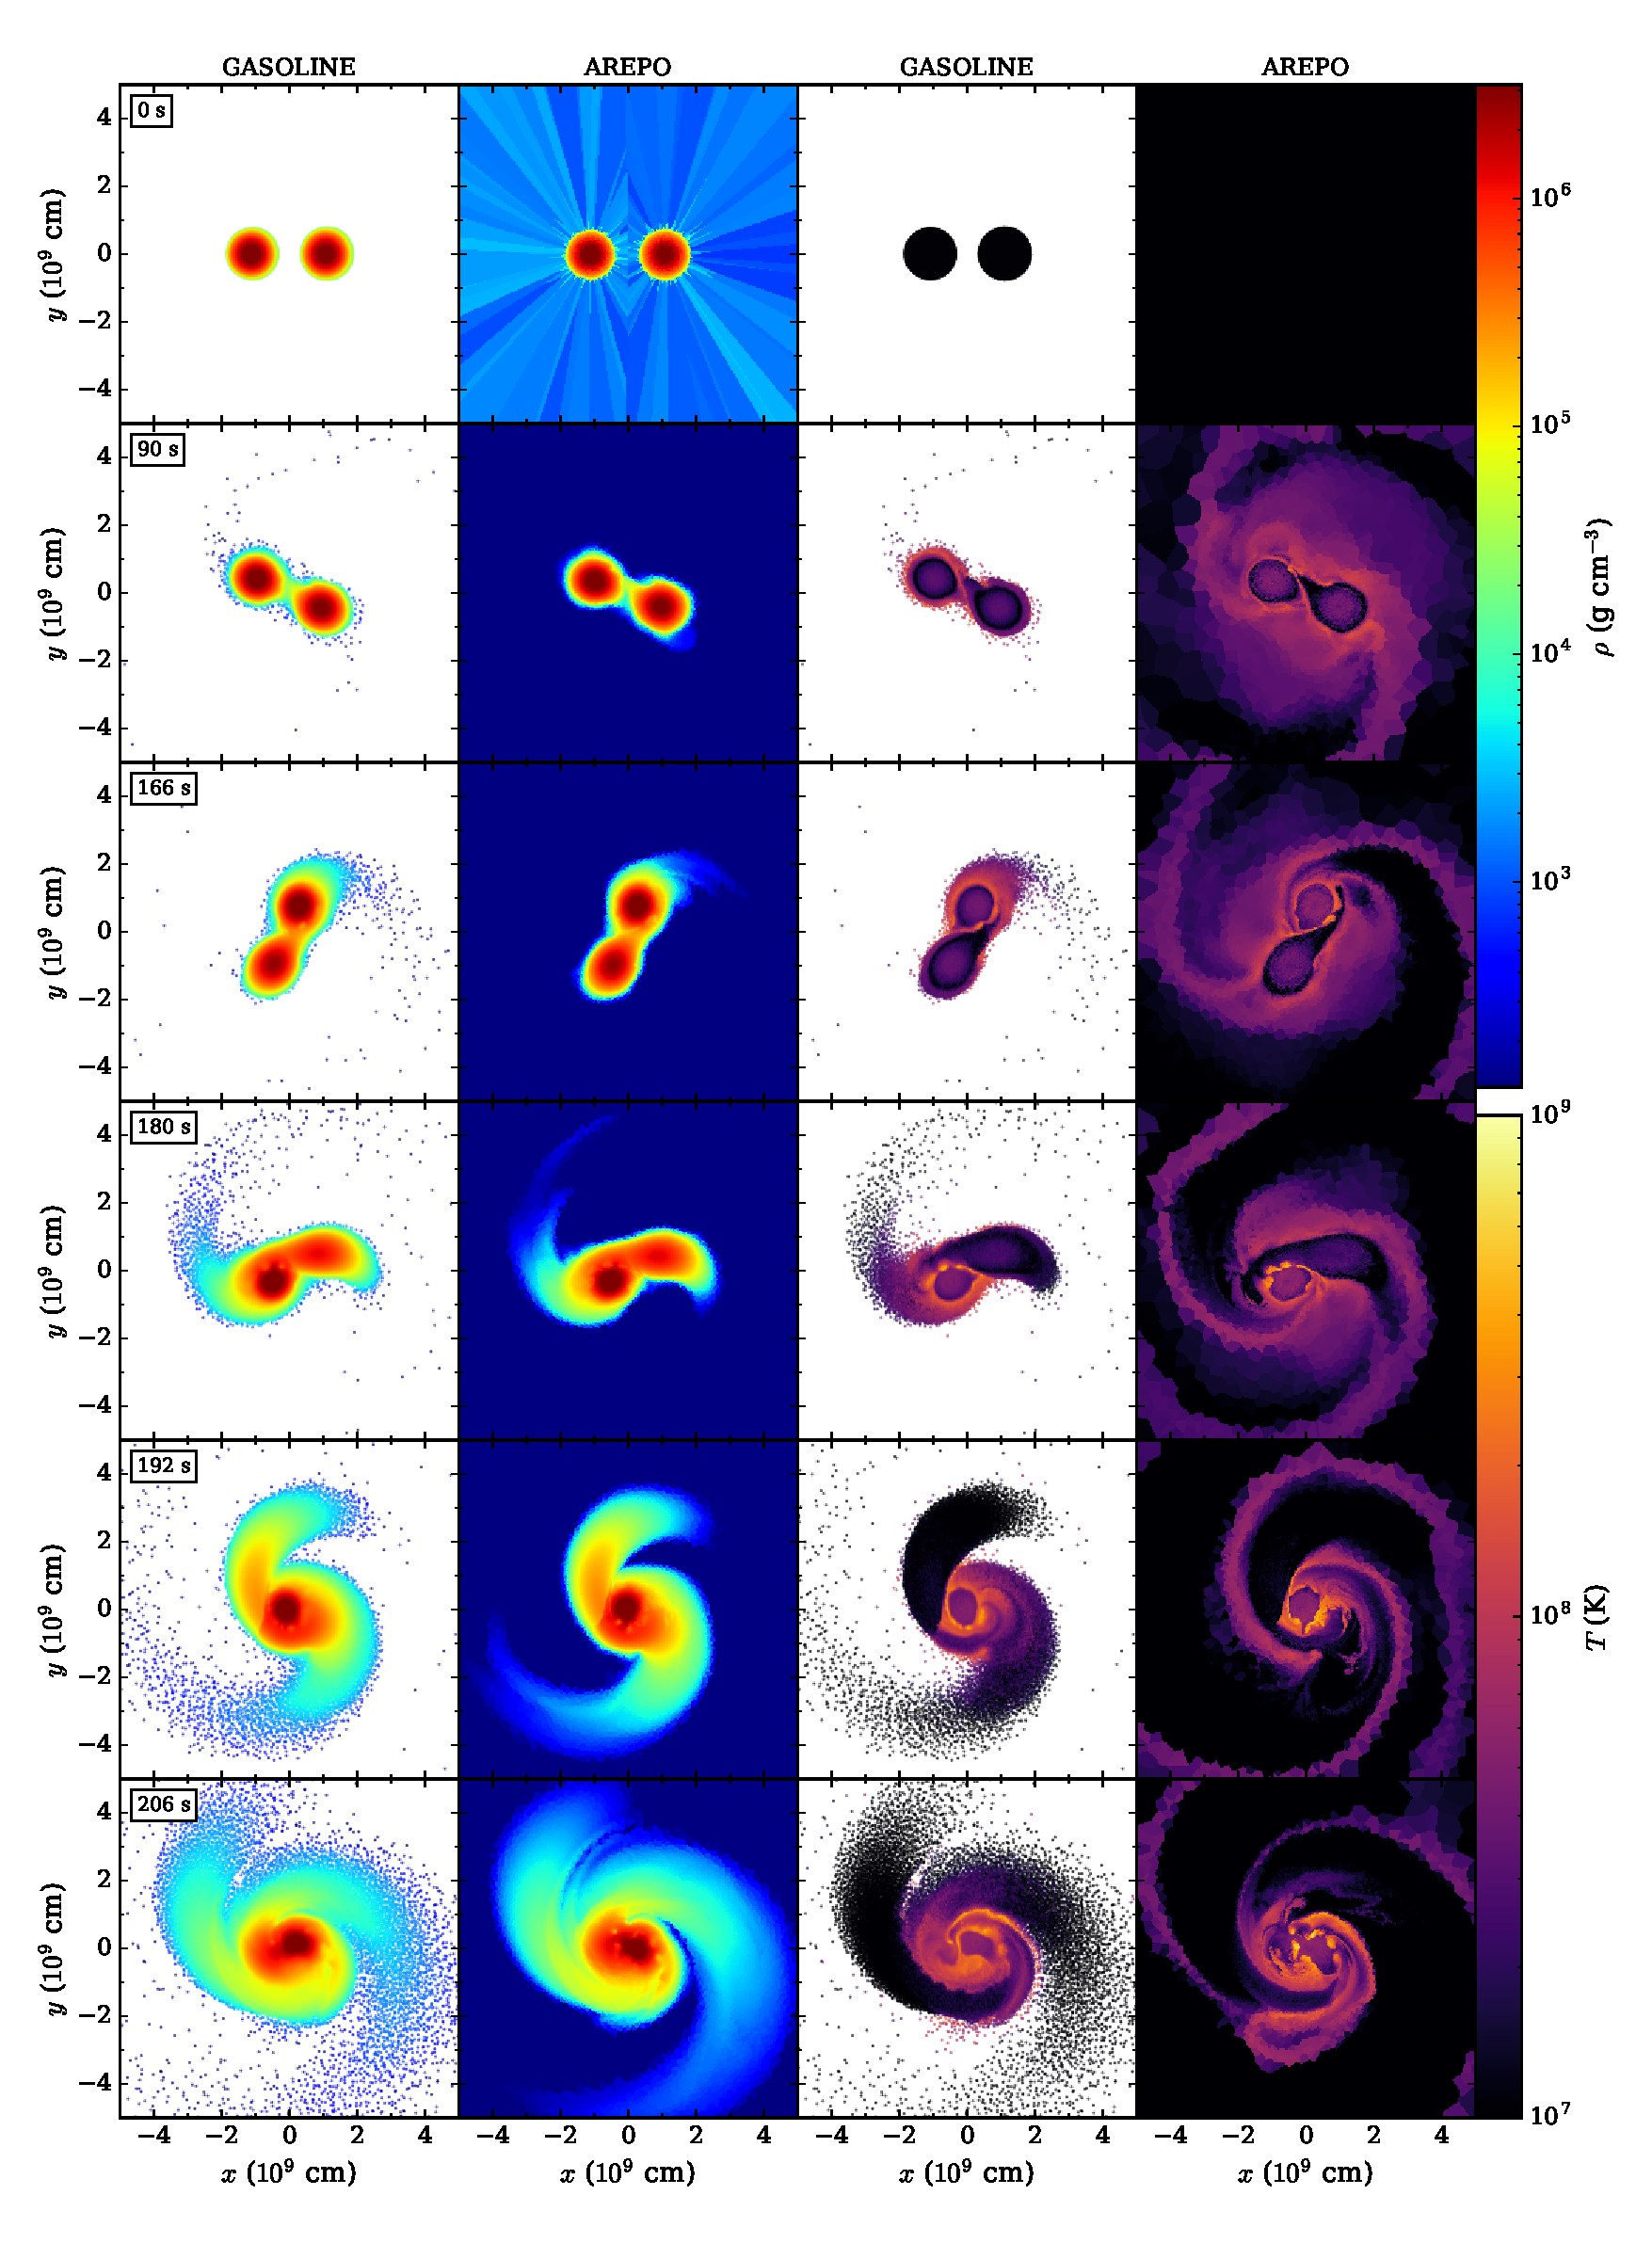
\includegraphics[angle=0,width=1.0\columnwidth]{chapter3_zhu+u/figures/snapshots1.pdf}
\end{figure}
\begin{figure}
\centering
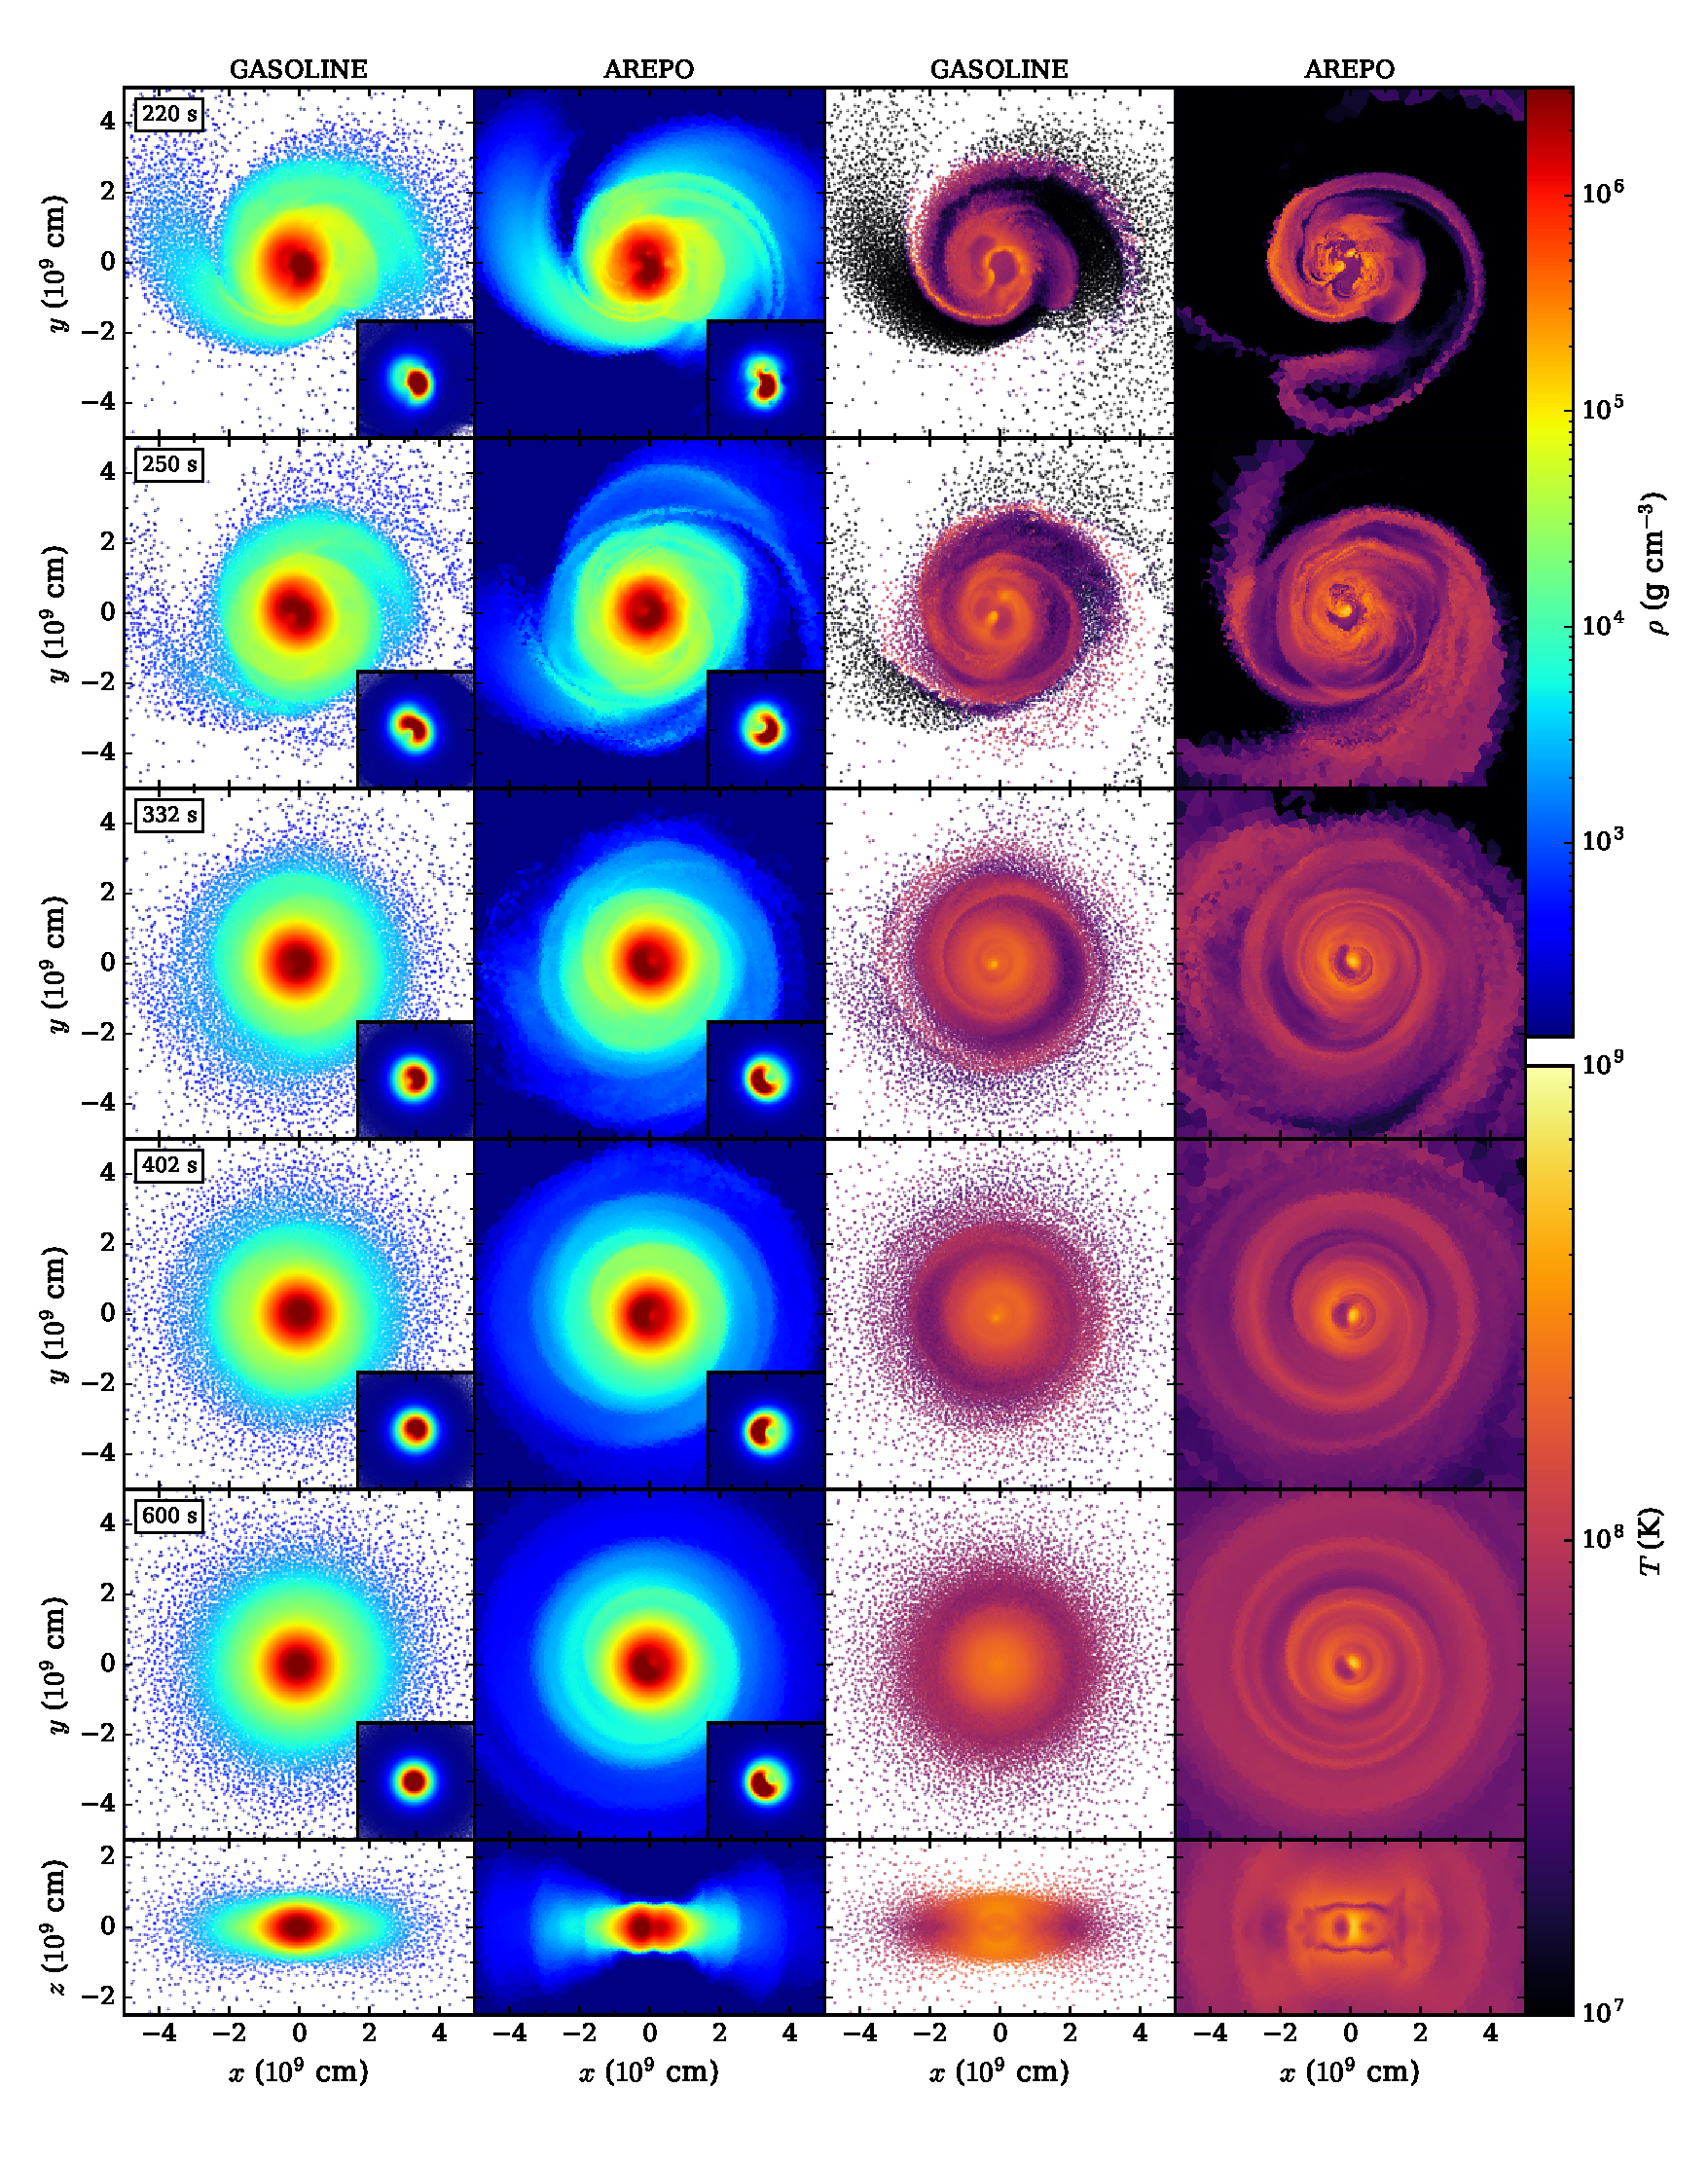
\includegraphics[angle=0,width=1.0\columnwidth]{chapter3_zhu+u/figures/snapshots2.pdf}
\caption{Series of equatorial ($xy$) plane density (left two columns) and temperature (right two columns) intensity plots for five snapshots in time (rows; the time for each snapshot is indicated at the top left of the density plots) during the \gasoline\ and \arepo\ simulations.  {\charles The pattern of radial ``spikes'' in the \arepo\ initial conditions density plot is an artifact of visualizing its irregular mesh (which was converted directly from \gasoline's initial conditions).}  Following coalescence of the WDs, linear inserts in the density plots depict the shape of the remnant core using the same spatial scale, but a linear color scale from $0$ to $3.1\times10^6\,\gcc$.  $xz$-plane plots are also included for the final snapshot.}
\label{fig:c3_diagslice}
\end{figure}

We now compare in detail our new \arepo\ simulation with a \gasoline\ one.  Fig. \ref{fig:c3_diagslice} compares snapshots of the two at various times.

The initial evolution of the two systems, shown in row 1 of Fig. \ref{fig:c3_diagslice}, is qualitatively similar.  Our initial conditions are approximate, so both stars immediately are tidally stretched by the binary potential, overshooting their Roche lobes in the process and transferring mass to each other in spurts.  This eventually dies down for the $0.65\,\Msun$ accretor, and becomes steady mass transfer for the $0.625\,\Msun$ donor, just prior to it becoming fully disrupted.  In reality, the donor WD should overflow first and begin a period of quasi-stable mass transfer over potentially dozens of orbits, and so our simulations, both of which experience full donor disruption in just a few orbits, overestimate the rate of early mass transfer \citep{dan+11}.

% To check the mach number, I compared the velocity of the stream (in the frame of the accretor's center 2.5x10^8 cm/s) with the sound-speed of the outer layers of the accretor (1.3x10^8 cm/s).  Hot atmosphere temperatures from paper_propsatdisruption(frame="early")

The accretion streams in both codes are traveling at supersonic speeds ($\mathcal{M} \approx 2$) relative to the accretor when they impact, and the resulting shocks cause rapid thermalization.  By the time the donor is fully disrupted a hot atmosphere has formed around the accretor, with temperatures of $1.6 \times 10^8\,\mrm{K}$ in  \arepo\ and $1.9\times 10^8\,\mrm{K}$ in \gasoline\ -- both about a quarter of the virial temperature, $GM_am_P\mu/3R_ak_B \approx 7 \times 10^8\,\mrm{K}$ -- and densities of $1.8\times10^5\,\gcc$ and $2.3\times10^5\,\gcc$, respectively.  As can be seen in Fig. \ref{fig:c3_diagslice} row 1, \arepo's hot atmosphere is somewhat less extended and has more localized hotspots in temperature compared to the extended and uniform one in \gasoline.  This may be due to a combination of \arepo\ not oversmoothing the gradients within the atmosphere, and having superior spatial resolution for the same mass resolution.

% Note to self: M = 10 is cited by Guillochon et al. 2010 by comparing the Keplerian velocity to the local soundspeed.  I'm using the actual velocity compared to the soundspeed, which is apparently much lower.  At best, we can get M = 3.

As mass transfer continues to expand the donor and draw it closer to the accretor, eventually tidal forces between the two are strong enough to fully disrupt the donor, stretching it out into a thick stream of material that wraps around the accretor (see Fig. \ref{fig:c3_diagslice}, row {\charles 2}).  In both simulations, this occurs after $\sim3.6$ orbital periods of the initial binary, or $\sim180\,\mrm{s}$, by which time the donor has transferred $\sim0.05\,\Msun$ to the accretor.  During coalescence, both the density and temperature profiles appear very similar between the codes, and the destruction of the donor takes place over the same amount of time -- about one orbital period ($49.5\,\mrm{s}$).

%Just read the KH blob temperatures off from the intensity plots at the disruption time of t = 180 s.  Lengths and widths were manually measured from the intensity plots with a temperature range of [3e8 to 6e8] and averaged between the three blobs for each simulation.  Peak temperatures visually read out of each blob and averaged for reported values.

Once the donor is fully disrupted, and coalescence begins, a portion of it forms an accretion stream that slides across the accretor at supersonic speeds, creating a string of Kelvin-Helmholtz vortices.  In \arepo\ these vortices are markedly more pronounced, being both larger by $\sim30$\% in radius, and having a slightly higher temperature of $\sim5\times10^8$ K compared to \gasoline's $\sim4\times10^8$ K.  The stream continues to inspiral toward the center of the accretor, severely deforming the accretor while carrying the string of Kelvin-Helmholtz vortices toward the center of the system.  The two WDs have nearly equal masses, so material near the surface of the accretor is dredged up and mixes with the stream, and the shape of the accretor changes from a sphere into a crescent.  Meanwhile, the remainder of the donor material forms a thick sub-Keplerian disk around the accretor.  Coalescence is approximately complete when the average separation between material from the donor and accretor changes from its initial value of $2.2\times10^9\,\mrm{cm}$ to its equilibrium value of $\sim1\times10^8\,\mrm{cm}$.  We thus estimate the time when coalescence is complete, \tcoal, by determining the time when average donor-accretor separation reaches a tenth of its initial value.  We find $\tcoal = 228\,\mrm{s}$ for \gasoline, and $220\,\mrm{s}$ for \arepo\ (roughly Fig. \ref{fig:c3_diagslice}, row 3).

\begin{figure}
\centering
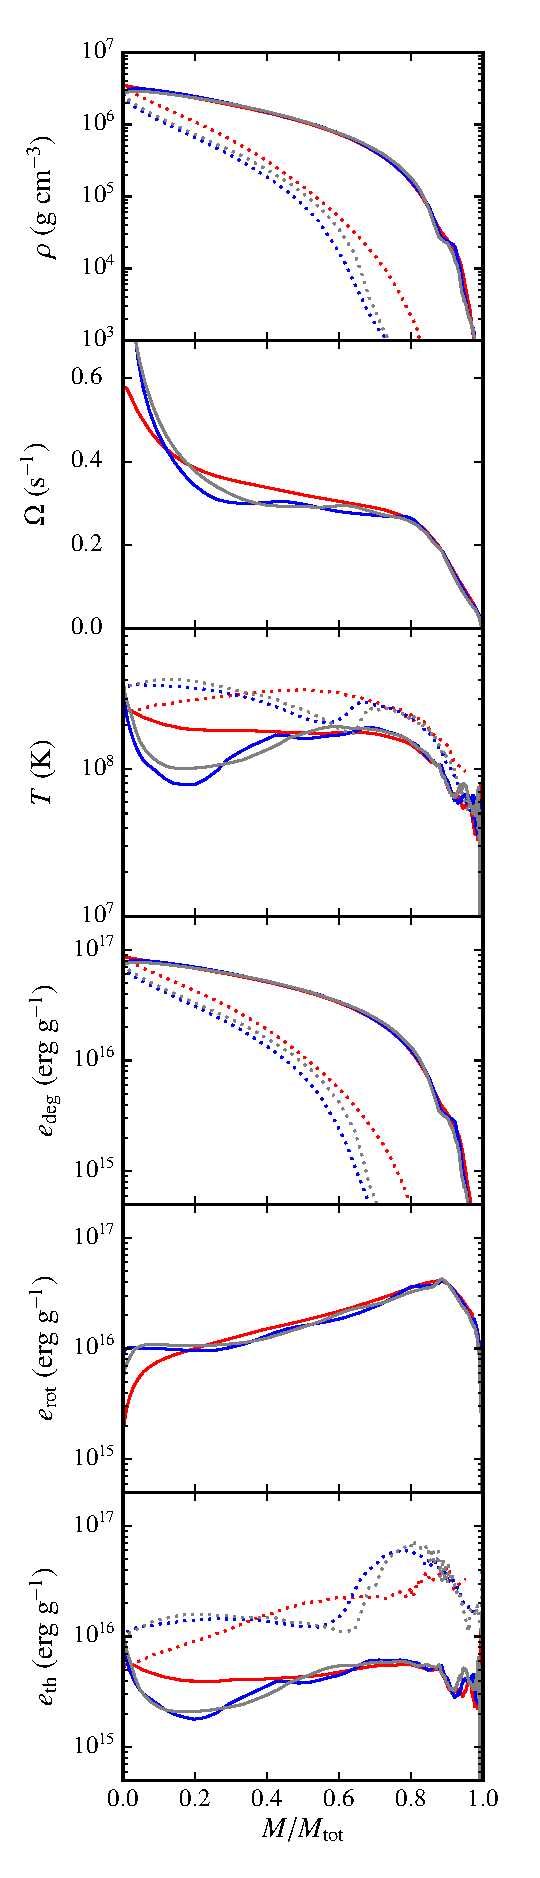
\includegraphics[angle=0,width=0.35\columnwidth]{chapter3_zhu+u/figures/curves.pdf}
\caption{Merger remnant profiles from the \gasoline\ (red), \arepo\ (blue) and \arepo\ MHD (gray; Ch. \ref{ch:ch4}) simulations $99\,\mrm{s}$ after coalescence (around row four of Fig. \ref{fig:c3_diagslice}).  The profiles are, from top to bottom, density $\rho$, angular rotation speed $\Omega$, temperature $T$, specific degeneracy energy  $e_{\rm deg}$, specific thermal energy $e_{\rm th}$, and specific rotational energy $e_{\rm rot}$, all as a function of the ratio of spherical enclosed to total mass $M/M_{\rm tot}$.  Solid lines represent profiles on the original binary's orbital plane, while dash-dotted lines represent profiles along the rotational axis.}
\label{fig:c3_curves}
\end{figure}

In Fig. \ref{fig:c3_curves}, we show profiles of density, temperature and energy for the merger remnants at $99\,\mrm{s}$ ($2$ orbital periods) after coalescence, roughly equivalent to row 4 of Fig. \ref{fig:c3_diagslice}.  Profiles both along the orbital plane of the original binary, or ``equatorial plane'' (solid lines) and rotational axis (dotted) are considered, and like in Ch. \ref{ch:ch2} we map (equatorial) $\varpi$ and (rotational) $z$ positions to the corresponding ratio of spherical enclosed mass to total mass $M/M_{\rm tot}$.  The equatorial profiles are axisymmetrically averaged, while the rotational axis ones are averaged from the profiles above and below the equatorial plane.  Overall, the two remnants have very similar structures: both feature a degeneracy-supported core surrounded by a rotationally supported thick disk along the equatorial plane and by a hot, thermally supported atmosphere along the axis of rotation.  Following Sec. \ref{sssec:c2_masstrends}, we find the disk mass $\Mdisk = 0.24\,\Msun$ and the core-envelope mass $\Mrem = 1.05\,\Msun$ in both simulations, though we note that the core-envelope also has substantial rotational support throughout.\footnote{The mass of material whose specific degeneracy energy is $>50$\% of their total specific energy is $\sim0.8\,\Msun$ in both simulations, as it is in Ch. \ref{ch:ch4}.}  Both remnants' total internal energies ($1.5\times10^{50}\,\mrm{erg}$) are also identically divided into $\sim30$\% rotational, $\sim10$\% thermal and $\sim60$\% degeneracy energy.  One minor difference between the two codes is the total amount of material unbound by the merger -- $1.4\times10^{-3}$ \Msun\ in \gasoline, and $5.0\times10^{-4}$ \Msun\ in \arepo\ -- though this value is much smaller and harder to constrain than the bulk values above.

% The unbound values take total energy into account, not just kinetic!

% Values below read off Fig fig:curves using ipython.  If you just look at the 1000 densest particles/cells, the density is 4e6 gcc (from snapshots 99 sec after coalescence).

The simulations' profiles in Fig. \ref{fig:c3_curves} are likewise very similar in shape to one another: both, for example, have a peak density of $\sim3\times10^6\,\gcc$ and a large fraction of their mass rotating nearly rigidly at $\sim0.3\,\psec$.  We also show the \arepo\ MHD simulation from Ch. \ref{ch:ch4} in grey, and find it is similar as well, indicating that the dramatic field amplification seen in that chapter leads only to minor changes in the \textit{hydrodynamics} of the merger.  The greatest discrepancy is in the temperature at small $M/M_{\rm tot}$: it is a factor of $\sim2$ smaller in the \arepo\ simulation than in the \gasoline\ one.

% Used max values from paper_cicomp_hotmix(res="high"), double checked by examining images.  Void size obtained from examining images.  Gasoline final temperature obtained by averaging temperature of material >1e5 gcc in the 100000.ascii snapshot; structure obtained by examining xy AND xz temperature structures for snapshots after 100000.ascii.

% Pattern speed determined by watching movies and timing the spiral wave and crescent; base of spiral determined using paper_spiralwave()

That discrepancy, however, reflects a growing difference visible in rows 4 - 6 of Fig. \ref{fig:c3_diagslice}.  Just after coalescence, the center of the merger remnant in both simulations is clearly divided between a dense and cold crescent-shaped region, formed from the perturbed accretor WD, and a low-density void that is an order of magnitude hotter, formed by material roughly evenly mixed between donor and accretor (this void appears as a column in the $xz$ plots of Fig. \ref{fig:c3_diagslice}).  $99\,\mrm{s}$ after coalescense, the hot void has a temperature of $\sim6\times10^8\,\mrm{K}$ in both codes, but the \arepo\ void is $\sim80$\% larger in radius and slightly less dense at $\sim1.5\times10^6\,\gcc$ versus \gasoline's $\sim2\times10^6\,\gcc$.  The cold crescent, meanwhile, has a density of $\sim4\times10^6\,\gcc$ in both codes, but has a temperature of $\sim2\times10^8\,\mrm{K}$ in \gasoline\ versus $\sim5\times10^7\,\mrm{K}$ in \arepo.  Over the next several hundred seconds, the \gasoline\ remnant's crescent becomes axisymmetric (see the linear inserts in Fig. \ref{fig:c3_diagslice}), eliminating the hot void in the process; material from the void moves off of the equatorial plane to form two $\sim3.5\times10^8\,\mrm{K}$ hotspots along the rotational axis (row 6 of Fig. \ref{fig:c3_diagslice}).  By $t\approx500\,\mrm{s}$, the \gasoline\ remnant structure -- an oblate spheroidal core with a roughly uniform temperature of $\sim 2 \times 10^8\,\mrm{K}$ (outside of the hotspots) surrounded by a stubby disk -- has stopped changing on a hydrodynamic timescale (roughly equal to one binary orbital period).  \arepo, on the other hand, maintains the distinction between the crescent and void, and consequently remains non-axisymmetric until the end of the simulation at $1000\,\mrm{s}$.  The system's center of rotation and mass are at the midpoint along the boundary between the crescent and void, and the dense crescent revolves around this point (rather than spinning about it).  This generates a lopsided gravitational potential that perturbs the surrounding disk, launching an $m = 1$ one-armed spiral wave into the surrounding medium.  The pattern speed is $\Omega_p \approx 0.4\,\mrm{s}^{-1}$ (as is the angular speed of the crescent), and the base of the spiral wave is at $\varpi \approx 1.5\times10^9\,\mrm{cm}$, where $\Omega \approx 0.2\,\mrm{s}^{-1}$ -- in 2:1 resonance with the crescent.

\begin{figure}
\centering
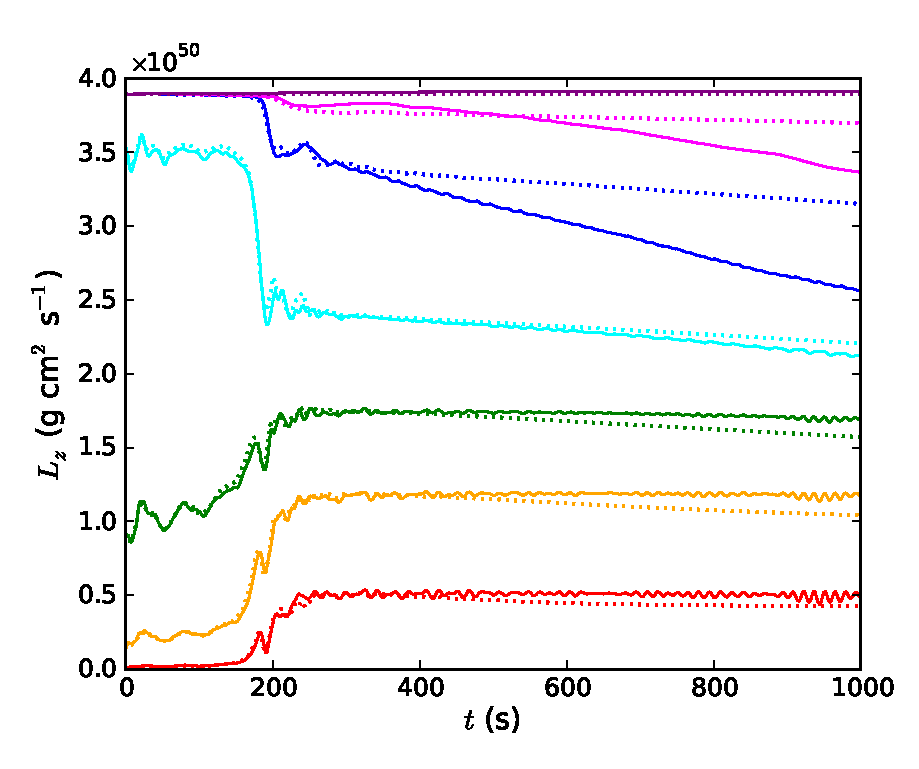
\includegraphics[angle=0,width=0.6\columnwidth]{chapter3_zhu+u/figures/Lz.pdf}
\caption{Time evolution of $z$-axis angular momentum \Lz\ for \arepo\ (solid lines) and \gasoline\ (dashed) simulations.  The purple line represents total \Lz, while the others represent angular momentum within concentric cylinders aligned along the rotation axis and with radii $\varpi = 5\times10^8$ (red), $7.5\times10^8$ (yellow), $1\times10^9$ (green), $1.5\times10^9$ (cyan), $3\times10^9$ (blue) and $6\times10^9\,\mrm{cm}$ (magenta).}
\label{fig:c3_angmo}
\end{figure}

Since spiral waves can transport angular momentum, we show in Fig. \ref{fig:c3_angmo} the evolution of $z$-axis angular momentum \Lz\ within concentric cylinders centered on the rotational axis for the two simulations.  We see that all cylinders slowly lose angular momentum after coalescence in the \gasoline\ simulation, consistent with the effect of artificial viscosity.  In \arepo, $\Lz(\varpi < 3\times10^9\,\mrm{cm})$ decreases at a rate of $d\Lz/dt = 1.2\times10^{47}\,\mrm{g}\,\mrm{cm}^2\,\mrm{s}^{-2}$ (compared to $3.3\times10^{46}\,\mrm{g}\,\mrm{cm}^2\,\mrm{s}^{-2}$ in \gasoline), reflecting the wave's angular momentum transport.  Applying Eqn. \ref{eq:c3_angmobalance} to the cylinder, we estimate around $\sim85$\% of this decrease can be accounted for by advection, suggesting the spiral wave transports angular momentum through Reynolds stresses (rather than gravitational torque; \citealt{kratl16}).  The angular momentum within \innercyl\ decreases by $\sim5$\% by the end of the simulation at $t = 1000\,\mrm{s}$, but the loss of angular momentum in the disk also results in the enclosed mass within \innercyl\ increasing by $0.02\,\Msun$ over the same timeframe.  In fact, the remnant disk has transported about half of its angular momentum to much larger distances by this time; the corresponding timescale is roughly equal to that for an $\alpha$-viscosity disk with $\alpha \sim 10^{-1}$.  For comparison, \cite{ji+13} simulate the magnetically-mediated viscous evolution of a $0.6-0.6\,\Msun$ merger remnant, and find angular momentum transport at a rate equivalent to an $\alpha = 10^{-2}$ disk, an order of magnitude smaller.  At $t = 1000\,\mrm{s}$, \arepo's void has shrunk by about a quarter of its initial radius, but the remnant core remains non-axisymmetric and the spiral wave persists, and so angular momentum transport should continue on a hydrodynamic timescale beyond the end of the simulation.

% Cold interface temperature obtained by eyeballing xz temperature map of snapshot_300 at standard resolution.

{\charles Preliminary attempts to carry the simulation even further in time in \arepo, however, have been stymied by the formation of a cold layer along the poles of the remnant following coalescence, which can be seen in the \arepo\ $xz$-plane temperature plot in Fig. \ref{fig:c3_diagslice}.  While the temperature of this layer is $\sim6\times10^7\,\mrm{K}$ for most of post-merger evolution, portions of it spuriously drop below $10^7\,\mrm{K}$ after $\sim1000\,\mrm{s}$.  The layer eventually expands to encompass the interface between the remnant core and disk when $t \gtrsim 2000\,\mrm{s}$.  The appearance of this layer, which becomes spuriously cold at $t \lesssim600\,\mrm{s}$ at the lower-resolution simulations in Sec. \ref{ssec:c3_restest}, is troubling, and suggests that \arepo\ must be further refined before the full hydrodynamic spin-down of the remnant can be simulated.  We therefore caution that the quantiative details of post-coalescence evolution discussed above may not be accurate, particularly close to the end of the simulation.}

%(since our highest resolution run in Sec. \ref{ssec:c3_restest} does not develop this issue) our qualitative results are more robust.  THIS ISN'T REALLY TRUE


%Under both codes, the remnant core is a cresent-shaped object off of the centre of rotation, flanked on one side by a low-density hot void, and therefore features a prominent $m = 1$ non-axisymmetric mode that we expect to either gravitationally torque or hydrodynamically stir the surrounding medium.  Disturbances generated by the core will naturally be stretched out into a trailing spiral pattern due to the differential rotation of the sub-Keplerian disk.

%\arepo, on the other hand, maintains the integrity of the cresent and void for hundreds of seconds.  In the high-resolution simulation, by $t = 200$ s, a single spiral with a $\delta \rho/\left\langle\rho\right\rangle$ of $\sim1$ and Mach number $\mathcal{M} \approx 2$ is generated, either through ram pressure, tides, or by a combination of the two, near the transition between the remnant core and disk.  Once generated, they hydrodynamically transport angular momentum outward before disappearing past $10^{10}$ cm, accounting for the strong \Lzinner\ loss seen in Fig. \ref{fig:angmo}.  Some dissipation occurs before the shock reaches $10^{10}$ cm, though, as we also find an outward mass flux throughout the entire disk, and a gain in angular momentum for material past $\sim3\times10^9$ cm.  These shocks also do not propagate only along the mid-disk: they trace out expanding semicircular arcs in the $r_\mrm{xy}-z$ plane, spreading material beyond the plane of the disk in a fan shape.

%\arepo, on the other hand, maintains the coherency of its void over hundreds of seconds as the torus of dense material deforms into a crescent and hydrodynamically launches a single spiral wave into the surrounding medium.  Over time, this spiral wave transports angular momentum away from the core, allowing the crescent to sink toward the remnant center of mass.  This is radically different than what we see in \gasoline, and has not been reported by other SPH simulation works, which suggests that there is a phase of hydrodynamic evolution following coalescence that is not properly captured by traditional SPH.  Unfortunately, issues with angular momentum conservation in \arepo\ prevent us from reliably following this post-merger hydrodynamic evolution further than a few hundred seconds, and we cannot definitely say if the remnant core is able to lose much of its angular momentum via spiral waves.  This issue is further discussed in Sec. \ref{ssec:pmeloss}.

%We have attempted to extend this simulation by several thousand seconds to probe the long-term stability of the remnant's structure, but find instead the spontaneous development of a dense $<10^7\,\mrm{K}$ layer (much colder than any material surrounding it) at the boundary between the remnant core and disk.  
